\documentclass{article}
\usepackage[utf8]{inputenc}
\usepackage{graphicx}
\graphicspath{ {./images/} }

\title{Upside: Understanding and Coping with Emotions}
\author{Sophia Abolore, Michelle Chernyi, Umayrah Chonee, Emily Chang }
\date{April 2021}

\begin{document}

    \maketitle


    \section{Introduction}

    In Psychology, emotions are defined as complex states of feeling that can result in physical and psychological changes that influence our thoughts and behaviours ("What is mental health?", n.d.). Most people experience a series of many different emotions but do not really understand what those emotions mean, the effects they may have physically and psychologically, and may not even know how to approach them. Moreover, some people may approach those emotions in a destructive way through their coping mechanisms. This project is founded on the idea that there are no good or bad emotions, but that there are good and bad ways of dealing with those emotions. Through this project, we will try to answer the question: {\bf how can we help people process and deal with their emotions in a healthy and non-destructive way based on the coping mechanisms that work the best for them.}\\

    We will answer this question by creating an interactive user interface and we will use a data set containing ten of the most experienced emotions. We will provide valuable information on the emotions such as their descriptions, their causes, their physical and psychological side effects, and most importantly the healthiest ways to deal with those emotions. The interface will allow users to go through the information associated with the emotion they are currently experiencing, keep track of which of the suggested coping mechanisms work for them, add their own preferred coping mechanisms to the list, and document their feelings and experiences with each emotion through the form of a journal that can be referenced back to. Additionally, they will be able to keep track of which of their personal coping mechanisms are unhealthy as well as, keep track of when they last used an unhealthy mechanism to cope. All of this information is stored so that the next time the user is experiencing a certain emotion, the coping mechanisms they have computed for that emotion are suggested to them. \\

    In addition, the user will be able to see the journal entries documented for that specific coping mechanism and potentially make changes to their list of coping mechanisms based on the entries or simply reflect back on them. Once the user labels one of their coping mechanisms as bad, a good coping mechanism is suggested instead. As well, there is a tracker which can be started by the user that keeps track of the last time they used an unhealthy copy mechanism. The idea is that over time, the user will have access to a wide range of coping mechanisms that work the best for them as well as be able to identify which coping mechanisms are healthy and which are unhealthy. They will be able to use these coping mechanisms time and again to manage their complex feelings. Moreover, the users will have a better understanding of each emotion and the reasons why they are experiencing them through the information provided. This will raise the users’ emotional awareness and will help them through their journey.


    \section{Description of Datasets}

    Our program uses a dataset of 10 emotions, and a corresponding description, list of causes, biological/psychological examination and list of coping mechanisms, for each emotion. The header of the csv file consists of:
    \begin{enumerate}
        \item Emotion
        \item Description
        \item Cause
        \item What’s Happening
        \item Coping Mechanisms\\
    \end{enumerate}


    The “Emotion” column consists of the names of each emotion, namely sadness, fear, vulnerability, exhaustion, envy, jealousy, anger, stress, anxiousness and procrastination. The “Description” column consists of strings that provide a definition of each of the featured emotions. The “Causes” column also comprises strings that represent some potential causes of each emotion. The “What’s happening” column consists of strings that provide a physiological or psychological description of the emotions' influence on people. The “Coping Mechanisms” column is made up of strings containing lists of various healthy coping mechanisms users can use to deal with the emotion they are experiencing, this string will also be split to separate each coping mechanism in our computations.\\

    In addition to this our project generates a dataset of journal entries based on the entries recorded by the users. Each row of the csv file contains the name of the emotion the user is journaling about in the first column and the journals entered by that user in the second column. \\

    This project also generates a dataset of time in a CSV file format. The dataset uses 3 columns: started, day, and past time. Started indicates whether the user pressed the button ‘start’, day indicates how many days have passed since the start button was pressed, and past time indicates the last date on which the user pressed the start button. This information gets replaced every time the user presses on start again. If the user pressed restart but has not pressed start yet, the started column will have ‘no’, the days column will have ‘0’ and the past time will be blank.


    \section{Computational Overview}
    Our project uses psychology research about emotions and relevant information about these emotions including a description, a list of causes, a list of effects, and a list of coping mechanisms. In order to display and use this information, a graph with all the information was created, where every emotion is a vertex with edges to the corresponding description vertex, causes vertex, effects vertex, and coping mechanisms vertices which can be neighbours of multiple emotions. This graph is then mutated based on user input and information is extracted from the graph to display to the user.\\

    \begin{center}
        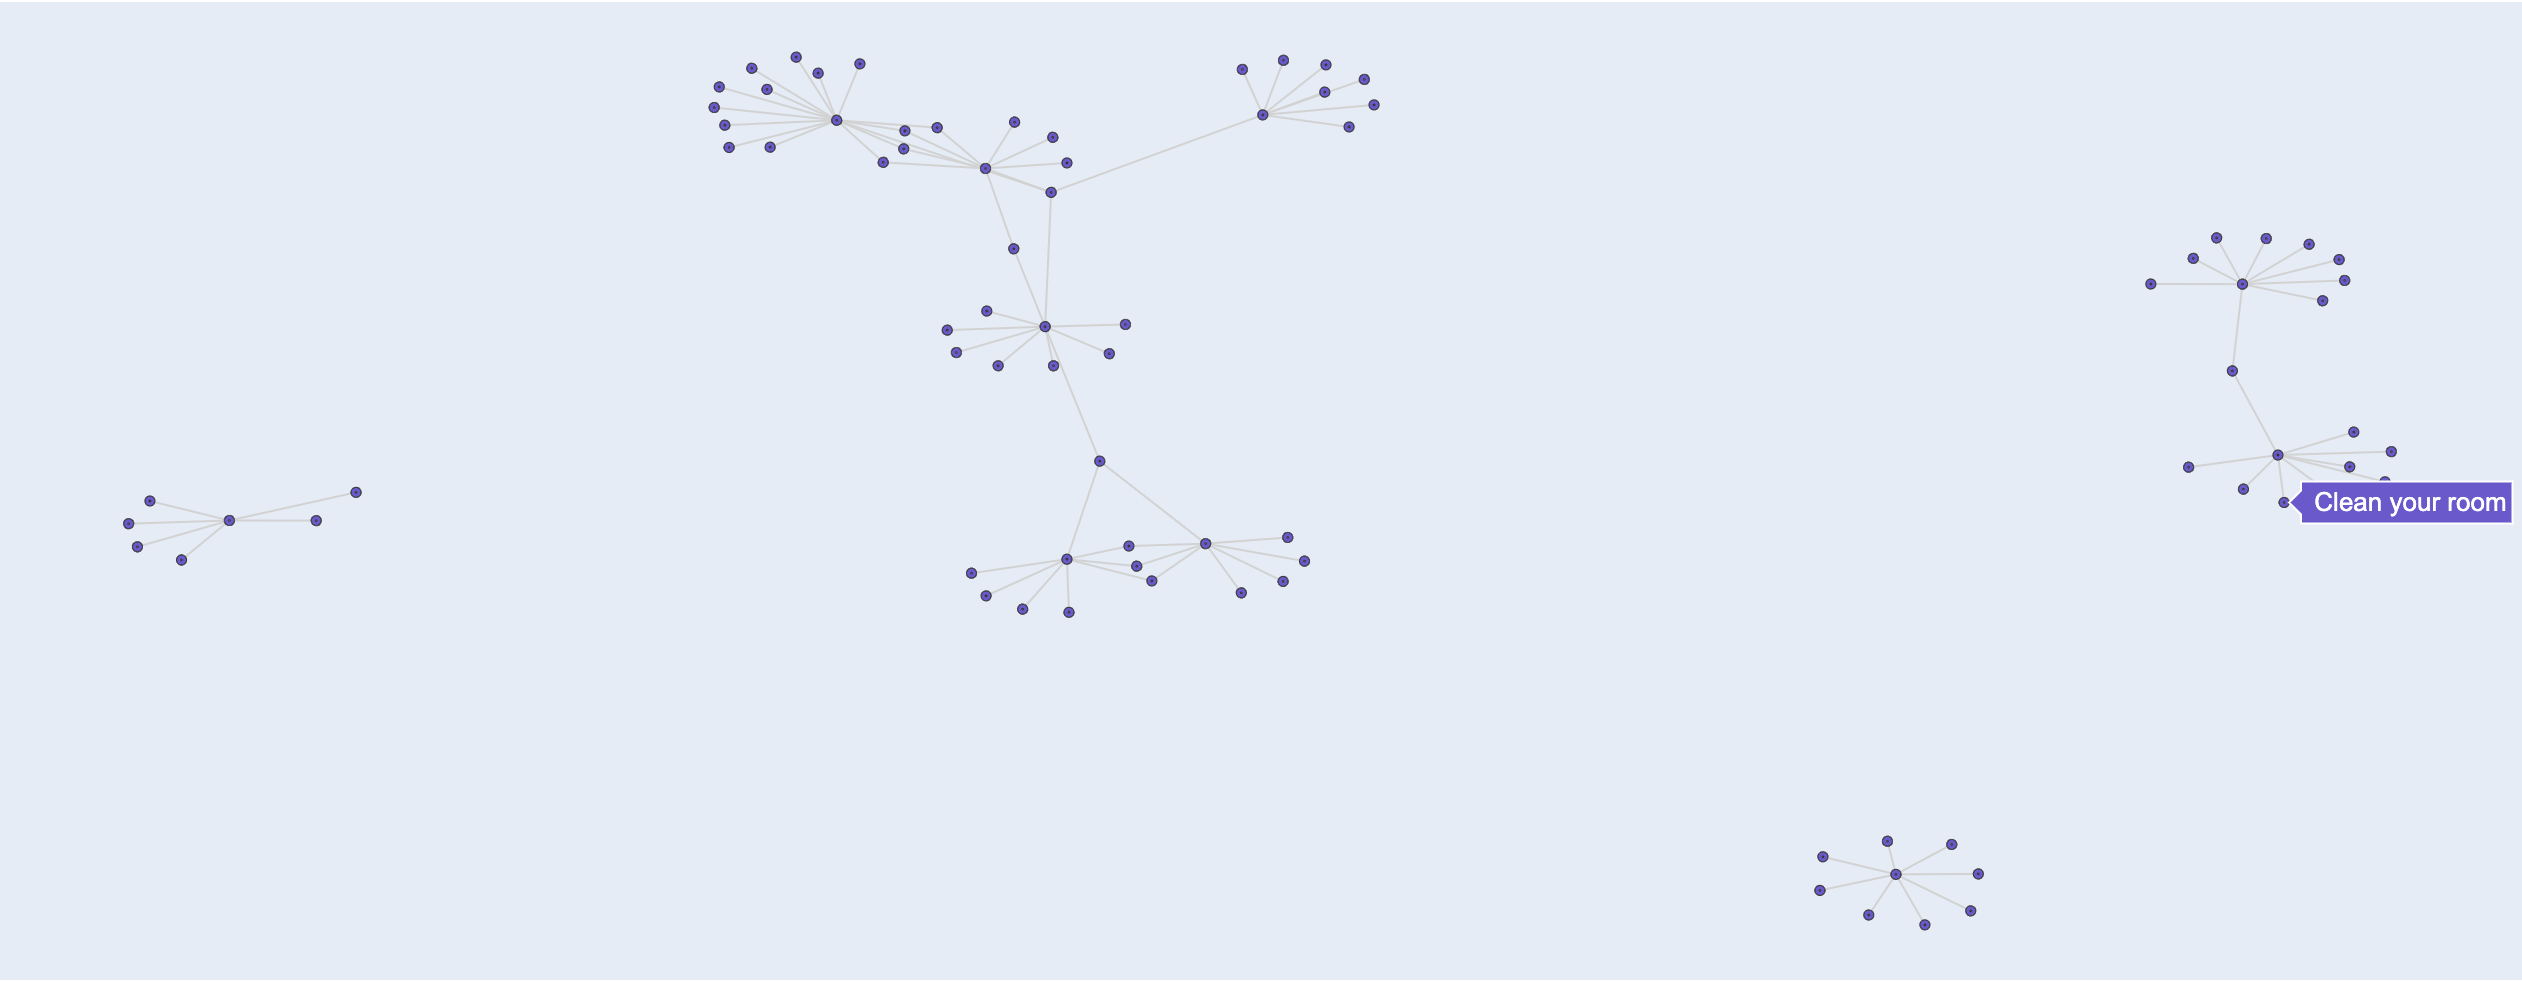
\includegraphics[width=12cm,height=9cm]{Images/graph.png}
    \end{center}
    The computations done on the graph mainly include building the graph and mutating or searching through it.
    load\_emotion\_graph takes the emotions csv and journal entries csv as the inputs and creates a graph object using the methods, add\_vertex, get\_all\_vertices, and add\_edge. \\

    Another computation is recommend\_coping\_mechanism which uses a graph method, get\_neighbour\_by\_kind, to find the specific neighbour of an unhealthy coping mechanism, an emotion vertex, and then returns one of the (healthy) coping mechanism vertices adjacent to that emotion.

    \_submit\_clicked function mutates the graph both directly and indirectly. It adds user inputted text as a vertex to the graph with kind, ‘journal’, and creates an edge with the corresponding coping mechanism vertex. It also adds the journal entry into the journal entries csv file using a different function, \_save\_text. The function also takes the input “value”, a boolean that when false will use the graph method, change\_vertex\_rate to change the rate of the coping mechanism to False. Then, it will use the function edit\_file to replace the coping mechanisms of the specific inputted emotion with coping mechanisms rated True in the emotions csv file .This gets rid of all coping mechanisms with rating false from the emotions csv file and as a result from the graph. The function also creates the journal frame with the new journal included by calling function journal() (this has to do with the User Interface, which will be discussed later). \\

    One more major computation is done by the function \_insert\_mechanism. This function gets a user inputted healthy coping mechanism and adds it as a vertex adjacent to the inputted emotion. The coping mechanism is also added to the emotions csv using edit\_file  and the specifics frame is refreshed to now include the new coping mechanism using function specifics() if it is a healthy coping mechanism. If the user inputted an unhealthy coping mechanism the recommendation() function is called which will create a new recommendation frame displaying a healthy coping mechanism corresponding to the emotion adjacent to the unhealthy coping mechanism. \\


    The rest of the major functions/ classes are responsible for creating an interactive and visual interface for the user using a new library, tkinter. tkinter is used for GUI programming such as creating and using widgets. The module allows for GUI elements, specifically widgets including text boxes, labels, and buttons as well as user entry. We used many classes and functions from tkinter to create the user interface. We used tk.Tk to create the main window for the app. We used geometry() to create window size and title() to give the window a title. We used frame() to create a new page on the same window. We also used tk.label(), tk.Button(), tk.Radiobutton(), etc. to create labels and buttons on the windows. We used .place() to place the widgets in the location we desired. Lastly, we used the command class to call on a function when a button is pressed by the user. These are just a few examples of the functions and classes from tkinter we used.

    There are 6 classes used to create the user interface. An UpsideApp() class initializes the main window for the app. The StartPage class creates the first page of the app, with buttons for different emotions. It uses command class to call on function options() (when a user clicks on the button), which will open the next page based on the emotion inputted. The next page is the options page created by class Options() which creates a label and buttons for ‘description’, ‘effects’, ‘causes’, and ‘coping mechanisms’. The buttons have a command class which will call the function specifics() as well as a back button (seen on many other pages), which uses the controller (an attribute of the main class) to call the StartPage() (or calls on another function to bring back to a different page). In the specifics page, information extracted from the graph will be displayed. If specifics() called on kind = coping mechanism, among other buttons, a journal\_button will be displayed which will call on the journal() function. This function will open a new frame which allows for user input using tk.Text(). This text is used in \_submit\_clicked() function (discussed earlier). There is also a past\_entries\_button which calls on the function display\_journal(), which opens DisplayJournals() class. This class shows all journals written under an emotion passed into function, on a new frame. \\


    The library textwrap, library used to wrap and fill text, is also used, specifically for its ability to take a string and make it into a paragraph with every line at most a specific amount of characters long using textwrap.fill() \\

    The library PIL is used for image processing. Specifically we used ImageTk to make the image compatible with tkinter and Image to load the picture. \\

    The library pandas is used for analyzing and using data. We used pd to read csv files. \\

    The last aspect of our project is a habit tracker, where the user can keep track of when they have used bad coping mechanisms. There is a stopwatch that keeps track of how long it’s been since a bad coping mechanism was used. The habit tracker uses the class HabitTracker(), function habit\_tracker(), read\_time\_csv() function, start\_timer() function, and edit\_time\_csv() function. The habit tracker function uses read\_time\_csv() to read the time csv file, calculate how many days have passed, based on the amount of days on the file, the current date and the date on the file and then edit the time csv file, specifically the past time and days passed to this point, or changes days to 0 if started is False. The HabitTracker() class displays this information using labels and makes changes to the file (if start and restart buttons are pressed by the user) by calling start\_timer().


    \section{Obtaining Datasets and Running The Program}

    Download all files from MarkUs, including the datasets. The datasets should be extracted from the zip file and saved in a ‘data’ folder (if they don’t do so automatically). The data file must be on the same level as the Python files, as well as a png file. All files must be placed in a folder (if they don't do so automatically). Mark the "data" and "images" file as source root, as well as the project folder created. Also, ensure that your folders are named 'data' and 'Images'.\\

    When main.py is run, the program will start running. The TA should see a medium sized window appear with a picture that says “Upside”, a label that says, “what emotion are you feeling today?”, and 10 buttons with different emotions. The window should look like this:\\

    \begin{center}
        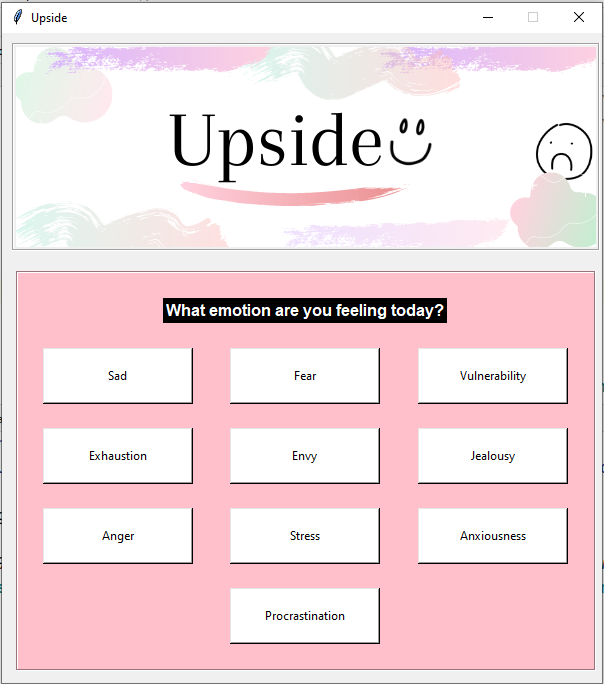
\includegraphics[width=11cm,height=12cm]{Images/upside.png}
    \end{center}

    To interact with the program the TA can do many things. First, the TA will choose an emotion, then they will see a screen with four buttons, ‘description’, ‘effects', 'causes', and 'coping mechanisms', that should look like this for example (in this example sad was picked): \\

    \begin{center}
        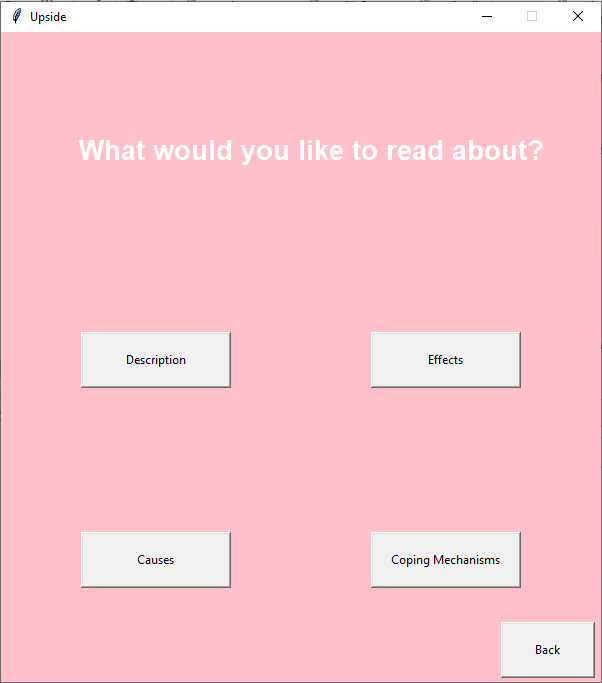
\includegraphics[width=11cm,height=12cm]{Images/options.png}
    \end{center}

    They can click on any of the buttons and receive information, once they read the information, they can can click on back button to go back to beginning page with emotions. if coping mechanisms button is clicked, the window will look similar to this:  \\

    \begin{center}
        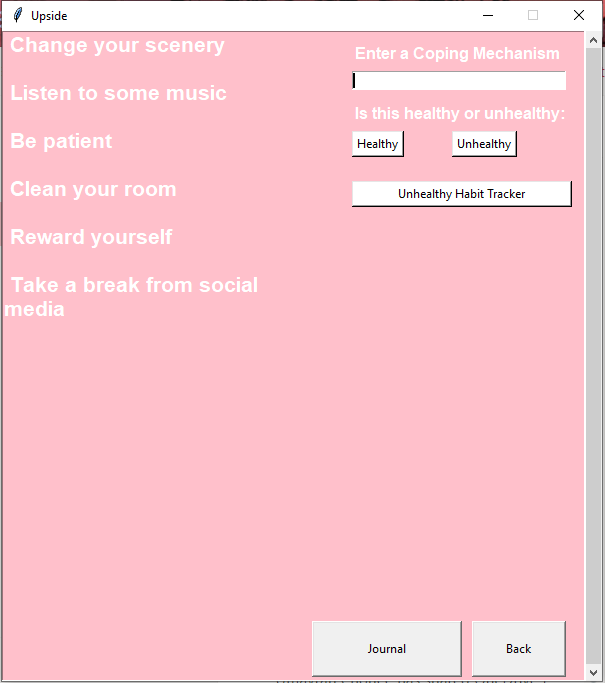
\includegraphics[width=11cm,height=12cm]{Images/copingmechanims.png}
    \end{center}

    In this window, the TA can enter coping mechanisms and pick if they are healthy or unhealthy. if the TA picks healthy, they should see the new coping mechanism in the list. If the TA pick unhealthy, they will be redirected to an alternative healthy coping mechanism and can click back to go back to the previous page. \\

    if the TA presses on unhealthy habit tracker, they should see a screen that prompts them to press start, when they press start they will see that they have not in engaged in bad coping mechanisms in 0 days. The program will keep track of the days passed even when the window is closed. Here is how it should look on day 0: \\

    \begin{center}
        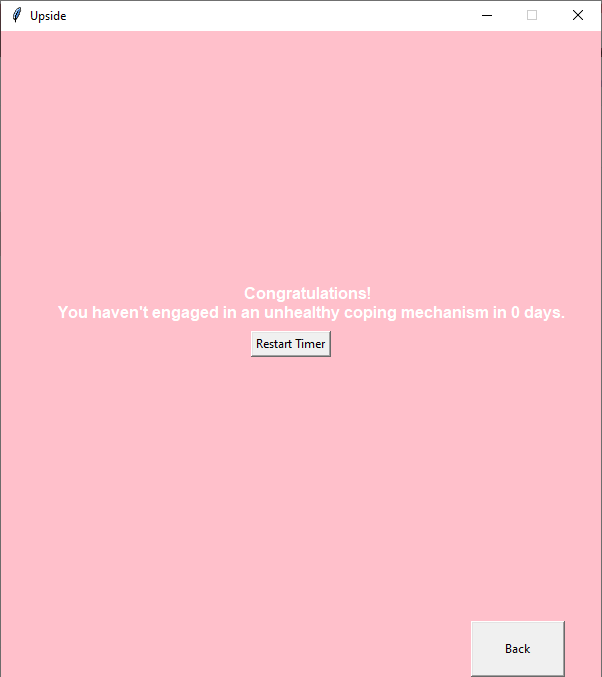
\includegraphics[width=11cm,height=12cm]{Images/timer.png}
    \end{center}

    Back on the coping mechanisms page, the TA can also press on journal. There, they will need to pick a coping mechanism from the dropdown menu and then they can write a journal about it. The TA can then choose if the coping mechanism was useful. If they pick yes the journal will be saved to the journal entries and they will be able to see it if they pick the same coping mechanism again in the drop down menu and press on 'past journal entries'. If they pick no, the coping mechanism will be discarded and will no longer be in the list of coping mechanisms. The picture of the journal page can be seen below: \\

    \begin{center}
        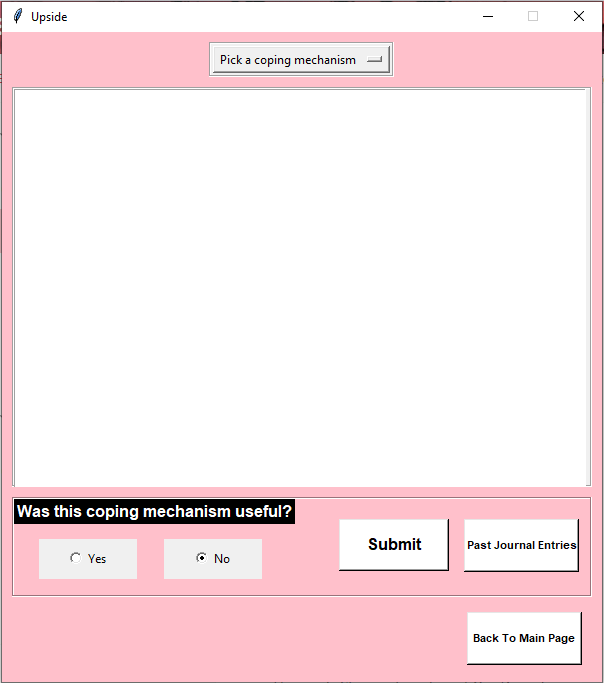
\includegraphics[width=11cm,height=12cm]{Images/journal.png}
    \end{center}


    \section{Changes To Our Plan}

    Our TA suggested inverting the proposed structure of our application and instead generating the emotion the user is experiencing based on their imputed symptoms, that way, since there’s a chance users might not know what emotion they are experiencing but know what symptoms are emerging. Although we thought this was a great idea and found the computation aspects of a suggestion tree/graph fascinating, this proposed model would not work well with the goals of our project, which are to facilitate knowledge and understanding of our emotions and explore ways to cope with them. The proposed model presents a diagnosis concept rather than a learning and growth concept and it is for that reason that we did not pursue that proposed model. However, we developed some ideas from the model and have made changes to our original plan.\\

    We’ve incorporated a suggestions element to our project. Now instead of users simply acknowledging their healthy and unhealthy coping mechanisms as we had initially planned, now when a user enters an unhealthy coping mechanism they will get a suggested healthy coping mechanism. In addition to this, users will now be able to document their experiences with those coping mechanisms through journal entries that are associated with specific coping mechanisms. We believe this will better facilitate a deeper understanding of the users relationship with their emotions and how they respond to different coping mechanisms. \\

    We also changed the data structure used in our application from a tree to a graph. We initially planned on creating a tree with the root “*”, similar to the second assignment, where the first level contains the names of the emotions, the second level contains the description, the third level contains the causes, the physical and psychological effects in the fourth level and the coping mechanisms in the final level. We were planning to mutate the tree after receiving user input by removing the leaves of the tree,which are the nodes containing the coping mechanisms and making them children of the root. However, we instead decided to use a graph with the name, description, causes and effects of each emotion represented by vertices connected to the specific emotion, and the cluster of information for each emotion, connected to other emotions by their coping mechanisms. \\

    We had initially planned to have a habit tracker that would keep track of how long it had been since the user had partook in each of their unhealthy coping mechanisms, however we came to the conclusion that all this information would be overwhelming to users and negatively impact their desire to overcome those unhealthy coping mechanisms. Instead we have a central unhealthy coping mechanism that keeps track of the last time the user has partaken in any unhealthy coping mechanism. This way users are aware of when they participate in unhealthy coping mechanisms without being overwhelmed by the many ways they may be doing so and losing their motivation. \\

    The last change we made was inserting the users imputed healthy coping mechanisms into the graph along with the coping mechanisms included in the dataset. In addition to this, instead of simply listing the coping mechanisms based on their ratings, coping mechanisms deemed unhelpful by the user are removed from the graph and no longer displayed as suggestions to the user.\\


    \section{Discussion}
    Our main goal with this project was to improve the mental health of users of our application by helping them with ways to understand and constructively deal with their emotions. We set out to answer the question of how we can help people process and deal with their emotions in a healthy and non-destructive way based on the coping mechanisms that work best for them. The results of our computational exploration provides a system that teaches the users of that system about the emotions they are experiencing as well as alerts them of the potential causes of that emotion and the side effects that they may experience as a consequence of that emotion. This provides users with a comprehensive view of their emotions and helps the users process their feelings effectively. In terms of helping users deal with those emotions we have numerous resources available through our collection of provided coping mechanisms, the ability of users to insert their own personal coping mechanisms, making users analyse whether or not their coping mechanisms are healthy, journalling their experiences in relation to their healthy coping mechanism and having a time tracker of when they last used an unhealthy coping mechanism. This all helps the user properly deal with their emotions in a healthy way that isn’t destructive to them in the long term. It is for this reason that the results of our computational exploration help answer our question. \\

    Limitations\\

    A significant limitation with our dataset is the fact that it only contains information for 10 emotions, whereas there are much more emotions experienced by people on a regular basis. Whereas these emotions are the most commonly experienced, our project would have benefitted from a data set with a wider variety of emotions as it would provide users with an even deeper understanding of their complex feelings. \\

    A computational limitation we experienced was the inability for us to regulate the imputed coping mechanisms, in the sense that the user could input multiple coping mechanisms that are either really similar or the exact same and spelt differently. Because we are unable to determine when a newly imputed coping mechanism is similar to a pre-existing coping mechanism, our application might become clustered with a list of very similar coping mechanisms, therefore lessening the effectiveness of the application. \\

    The final limitation of our application was the differences between our User Interface with tkinter depending on whether we were using a Mac or windows computer to run the program. Since most of the UI development took place on a Windows laptop, when we tried to run the program on one of our Mac laptops we noticed differences in the layout of the page, the visibility of texts and the colours of the buttons. We combatted this by trying adjusting the code for the UI on our Mac laptops and seeing if they were compatible with the Windows laptops. \\

    Some next steps for further exploration would definitely be including more emotions into the dataset, as well as providing descriptions for the coping mechanisms and adding citations for the descriptions and effects of each emotion with links to reputable sources that discuss those topics further. We would also like to include an artificial intelligence element to our project. When the user enters an unhealthy coping mechanism we don’t want to just suggest a coping mechanism based on the mechanisms that are adjacent to the coping mechanisms for that emotion, but generating coping mechanisms best suited to combat the unhealthy coping mechanism imputed by the user. \\

    Lastly we would like to include a social aspect to our project by enabling different users to interact with each other and try out coping mechanisms together as well as suggest coping mechanisms to others. This way the journey of users in mental wellness won’t be one they have to take by themselves.\\


    \section{Conclusion}

    Our project is only one way of promoting mental wellness and is far from a perfect approach at it, however it takes an approach that is deeply rooted in the understanding of these emotions, because there is strength in knowledge. By providing people with the understanding of their feelings and ways to cope with them we believe they will be equipped with the necessary tools of prioritizing their mental wellness. Although we experienced many setbacks, we were able to combat them and find alternatives to reach our desired destination. All in all, the creation of this project was a great learning experience as it not only provided us with insights into the different and real world ways data structures such as graphs are used, but it also helped us learn a lot about our emotions and ways to better our mental wellness.


    \section{References}
    -, A. (2020, March 24). Guilt and how it affects us. Retrieved April 20, 2021, from https://www.mindpathcare.com/guilt-affects-us/ \\

    8th, M., 1st, J., 14th, M., 16th, A., 29th, I., 23rd, R., . . . 7th, J. (2020, December 22). How to deal with jealousy:
    Overcoming overwhelming jealous feelings. Retrieved April 20, 2021, from https://www.psychalive.org/how-to-deal-with-jealousy/\\

    Amy Morin, L. (2020, August 03). Anger management techniques to calm you down fast. Retrieved April 20, 2021, from https://www.verywellmind.com/anger-management-strategies-4178870\\

    Anger management: 10 tips to tame your temper. (2020, February 29). Retrieved April 20, 2021, from https://www.mayoclinic.org/healthy-lifestyle/adult-health/in-depth/anger-management/art-20045434 \\

    Anger symptoms, causes and effects. (n.d.). Retrieved April 20, 2021, from https://www.psychguides.com/anger-management/ \\

    Anger. (n.d.). Retrieved April 20, 2021, from \\https://www.psychologytoday.com/ca/basics/anger \\

    Article by: John Riddle. (2020, February 21). Procrastination: Why we do it and what it says about our psyche. Retrieved April 20, 2021, from https://www.psycom.net/procrastination-why-we-do-it

    Article by: Sherry Amatenstein. (2021, January 05). 6 tips to Overcoming anxiety and phobias. Retrieved April 20, 2021, from https://www.psycom.net/facing-your-fear \\

    Attention. (n.d.). Retrieved April 20, 2021, from\\
    https://www.psychologytoday.com/us/basics/attention \\

    Augustine, A., & Larsen, R. (2011, April). Affect regulation and temporal discounting: Interactions between primed, state, and trait affect. Retrieved April 20, 2021, from https://www.ncbi.nlm.nih.gov/pubmed/21500908 \\

    Baeldung. (2020, December 09). What is an augmenting path? Retrieved April 20, 2021, from https://www.baeldung.com/cs/augmenting-path \\

    Barrett, H. (n.d.). How social media can affect your MOOD: Holland & Barrett. Retrieved April 20, 2021, from https://www.hollandandbarrett.com/the-health-hub/conditions/mental-health/how-social-media-can-affect-your-mood/ \\

    Boothby, S. (2017, April 13). How does music affect your mood and emotions. Retrieved April 20, 2021, from https://www.healthline.com/health-news/mental-listening-to-music-lifts-or-reinforces-mood-051713#2\\

    Brown University. (n.d.). Retrieved April 20, 2021, from https://www.brown.edu/campus-life/support/counseling-and-psychological-services/overcoming-procrastination \\

    Can mindfulness exercises help me? (2020, September 15). Retrieved April 20, 2021, from https://www.mayoclinic.org/healthy-lifestyle/consumer-health/in-depth/mindfulness-exercises/art-20046356 \\

    Cherry, K. (2020, June 29). Overview of the 6 major theories of emotion. Retrieved April 20, 2021, from https://www.verywellmind.com/theories-of-emotion-2795717 \\

    Cherry, K. (n.d.). What is procrastination? Retrieved April 20, 2021, from https://www.verywellmind.com/the-psychology-of-procrastination-2795944 \\

    Dr Elaine Ryan. (2020, May 09). Things that make you anxious; the things do not cause anxiety. Retrieved April 20, 2021, from https://mytherapist.ie/things-that-make-you-anxious/ \\

    Dropdown menus with TKINTER - Python Tkinter GUI TUTORIAL #18. (2019, April 30). Retrieved April 20, 2021, from \\https://www.youtube.com/watch?v=3E_fK5hCUnI \\

    ElSaady, A. (2016, December 05). 7 signs you're emotionally vulnerable. Retrieved April 20, 2021, from https://identity-mag.com/7-signs-youre-emotionally-vulnerable/ \\

    Emotional exhaustion: Causes, symptoms, risk factors, and prevention. (n.d.). Retrieved April 20, 2021, from \\https://www.medicalnewstoday.com/articles/323441#treatment-and-tips-for-recovery \\

    Envy - iresearchnet. (2016, January 22). Retrieved April 20, 2021, from https://psychology.iresearchnet.com/social-psychology/emotions/envy/ \\

    Fahkry, T. (2018, February 05). How to embrace vulnerability as your greatest strength. Retrieved April 20, 2021, from https://medium.com/the-mission/how-to-embrace-vulnerability-as-your-greatest-strength-d2ac2b80ba52 \\

    Fear: What happens in the brain and body? (n.d.). Retrieved April 20, 2021, from https://www.medicalnewstoday.com/articles/323492.php#1 \\

    Fritscher, L. (n.d.). The psychology behind fear. Retrieved April 20, 2021, from https://www.verywellmind.com/the-psychology-of-fear-2671696 \\

    Fuller, K. (2019, October 17). The difference between sadness and depression. Retrieved April 20, 2021, from https://www.psychologytoday.com/ca/blog/happiness-is-state-mind/201910/the-difference-between-sadness-and-depression \\

    Grande, D. (2019, February 24). Emotional vulnerability as the path to connection. Retrieved April 20, 2021, from https://www.psychologytoday.com/ca/blog/in-it-together/201902/emotional-vulnerability-the-path-connection \\

    Graphical user interfaces with tk¶. (n.d.). Retrieved April 20, 2021, from https://docs.python.org/3/library/tk.html \\

    Hill, S. E., & Buss, D. M. (2008). The evolutionary psychology of envy. Envy,60-70. doi:10.1093/acprof:oso/9780195327953.003.0004\\

    Holland, K. (2020, March 28). 11 anxiety triggers and how to identify and manage them. Retrieved April 20, 2021, from \\https://www.healthline.com/health/anxiety/anxiety-triggers#identifying-triggers \\

    Holland, K. (2020, September 03). Anxiety: Causes, symptoms, treatment, and more. Retrieved April 20, 2021, from https://www.healthline.com/health/anxiety#natural-remedies \\

    How to overcome fear and anxiety. (2020, August 10). Retrieved April 20, 2021, from https://www.mentalhealth.org.uk/publications/overcome-fear-anxiety \\

    Hughes, L. (2017, March 02). How to stop feeling anxious right now. Retrieved April 20, 2021, from https://www.webmd.com/mental-health/features/ways-to-reduce-anxiety \\

    Is vulnerability a choice? (2020, January 06). Retrieved April 20, 2021, from https://fs.blog/2020/01/vulnerability/ \\

    Jaffe, E. (2013, March 29). Why wait? The science BEHIND PROCRASTINATION. Retrieved April 20, 2021, from https://www.psychologicalscience.org/observer/why-wait-the-science-behind-procrastination \\

    Johansson, A. (2018, April 13). Why natural scenery improves your mood and makes you more productive. Retrieved April 20, 2021, from\\ https://www.nbcnews.com/better/health/why-natural-scenery-improves-your-mood-makes-you-more-productive-ncna860806 \\

    Kirmayer, M. (2017, November 28). How to cope when you're envious of a friend. Retrieved April 20, 2021, from https://www.psychologytoday.com/ca/blog/casual-close/201711/how-cope-when-you-re-envious-friend \\

    Konnikova, M. (2017, June 19). Can envy be good for you? Retrieved April 20, 2021, from https://www.newyorker.com/science/maria-konnikova/can-envy-be-good-for-you \\

    Kumar, B., & KumarEntrepreneur, B. (2021, January 11). Python Tkinter stopwatch (stopwatch source code in python). Retrieved April 20, 2021, from https://pythonguides.com/python-tkinter-stopwatch/ \\

    Lamia, M. (2013, July 13). Jealousy and envy: The emotions of comparison and contrast. Retrieved April 20, 2021, from \\https://www.psychologytoday.com/ca/blog/intense-emotions-and-strong-feelings/201307/ \\jealousy-and-envy-the-emotions-comparison-and \\

    Leahy, R. (2008, May 19). Jealousy is a killer: How to break free from your jealousy. Retrieved April 20, 2021, from https://www.psychologytoday.com/ca/blog/anxiety-files/200805/jealousy-is-killer-how-break-free-your-jealousy \\

    Learn Tkinter in 20 minutes. (2017, January 16). Retrieved April 20, 2021, from https://www.youtube.com/watch?v=\_lSNIrR1nZU&t=2s
    Lieberman, C. (2019, March 25). Why you procrastinate (it has nothing to do with self-control). Retrieved April 20, 2021, from https://www.nytimes.com/2019/03/25/smarter-living/why-you-procrastinate-it-has-nothing-to-do-with-self-control.html \\

    Lyness, D. (Ed.). (2015, August). Dealing with anger (for teens) - nemours kidshealth. Retrieved April 20, 2021, from https://kidshealth.org/en/teens/deal-with-anger.html \\

    MacDonald, F. (n.d.). This is what happens to your brain when you get your heart broken. Retrieved April 20, 2021, from https://www.sciencealert.com/this-is-what-happens-to-your-brain-when-you-get-your-heart-broken \\

    Melinda. (n.d.). Quick stress relief. Retrieved April 20, 2021, from \\ https://www.helpguide.org/articles/stress/quick-stress-relief.htm \\

    Michel, A. (2016, January 29). Burnout and the brain. Retrieved April 20, 2021, from https://www.psychologicalscience.org/observer/burnout-and-the-brain \\

    Morin, A. (2015, October 02). 6 reasons to treat yourself better. Retrieved April 20, 2021, from https://www.psychologytoday.com/us/blog/what-mentally-strong-people-dont-do/201510/6-reasons-treat-yourself-better \\

    Mullen, P., & Martin, J. (1994, January). Jealousy: A community study. Retrieved April 20, 2021, from https://www.ncbi.nlm.nih.gov/pubmed/8137108 \\

    Paige Fowler January 29, & Fowler, P. (2015, January 29). 7 health benefits of getting organized. Retrieved April 20, 2021, from \\https://www.shape.com/lifestyle/mind-and-body/how-cleaning-and-organizing-can-improve-your-physical-and-mental-health \\

    Pillow¶. (n.d.). Retrieved April 20, 2021, from \\https://pillow.readthedocs.io/en/stable/ \\

    Procrastination. (n.d.). Retrieved April 20, 2021, from \\https://www.google.ca/amp/s/www.psychologytoday.com/ca/basics/procrastination \\

    Psychology tools: What is anger? A secondary emotion. (2016, December 24). Retrieved April 20, 2021, from \\ https://healthypsych.com/psychology-tools-what-is-anger-a-secondary-emotion/ \\

    Publishing, H. (n.d.). Understanding the stress response. Retrieved April 20, 2021, from https://www.health.harvard.edu/staying-healthy/understanding-the-stress-response \\

    Python 3 - gui Programming (Tkinter). (n.d.). Retrieved April 20, 2021, from \\https://www.tutorialspoint.com/python3/python\_gui_programming.htm \\

    Real Python. (2021, April 03). Python gui programming with tkinter. Retrieved April 20, 2021, from https://realpython.com/python-gui-tkinter/ \\

    Real Python. (2021, April 03). Python gui programming with tkinter. Retrieved April 20, 2021, from https://realpython.com/python-gui-tkinter/#getting-user-input-with-entry-widgets \\

    Robinson, L. (n.d.). The mental health benefits of exercise. Retrieved April 20, 2021, from https://www.helpguide.org/articles/healthy-living/the-mental-health-benefits-of-exercise.htm \\

    Santos-Longhurst, A. (2018, October 26). Mental exhaustion: Definition, causes, symptoms, and treatment. Retrieved April 20, 2021, from \\ https://www.healthline.com/health/mental-exhaustion#overview \\

    Sasha0. (n.d.). Sasha0/timetracker. Retrieved April 20, 2021, from \\https://github.com/sasha0/timetracker/blob/master/timetracker/timetracker.py \\

    Sentdex. (2014, November 02). Multiple windows/frames in Tkinter GUI with Python - Tkinter TUTORIAL Python 3.4 p. 4. Retrieved April 20, 2021, from https://www.youtube.com/watch?v=jBUpjijYtCk \\

    Sicinski, A., & About The Author Adam Sicinski Adam is a life coach. (2018, December 10). How to Eliminate guilt that is slowly draining your life away. Retrieved April 20, 2021, from https://blog.iqmatrix.com/eliminate-guilt \\

    Stress: Signs, symptoms, management & prevention. (n.d.). Retrieved April 20, 2021, from https://my.clevelandclinic.org/health/articles/11874-stress \\

    Stress: Why does it happen and how can we manage it? (n.d.). Retrieved April 20, 2021, from https://www.medicalnewstoday.com/articles/145855 \\

    Team, G. (n.d.). Types of guilt. Retrieved April 20, 2021, from \\https://www.goodtherapy.org/learn-about-therapy/issues/guilt \\

    Textwrap - text wrapping and filling¶. (n.d.). Retrieved April 20, 2021, from https://docs.python.org/3/library/textwrap.html \\

    Wei, M. (2015, January 25). How to keep social media from complicating your relationship. Retrieved April 20, 2021, from \\ https://www.psychologytoday.com/ca/blog/urban-survival/201501/how-keep-social-media-complicating-your-relationship \\

    Weisberger, M. (2016, October 30). Scary science: How your body responds to fear. Retrieved April 20, 2021, from https://www.livescience.com/56691-the-science-of-fear.html \\

    What causes anxiety? 14 things that can make you feel anxious. (n.d.). Retrieved April 20, 2021, from https://www.webmd.com/anxiety-panic/guide/causes-anxiety \\

    What is mental health? (n.d.). Retrieved April 20, 2021, from \\https://www.mentalhealth.gov/basics/what-is-mental-health \\

    Why do i feel anxious and panicky? (n.d.). Retrieved April 20, 2021, from https://www.nhsinform.scot/healthy-living/mental-wellbeing/anxiety-and-panic/why-do-i-feel-anxious-and-panicky \\

    Williams, R. (2017, November 7). Anger as a basic emotion and its role in PERSONALITY building and pathological growth: The Neuroscientific, developmental and CLINICAL PERSPECTIVES. Retrieved April 20, 2021, from https://www.ncbi.nlm.nih.gov/pmc/articles/PMC5681963/ \\


\end{document}
